\documentclass[tikz]{standalone}
\usepackage[T1]{fontenc}
\usepackage[utf8]{inputenc}
\usepackage{pgfplots}
\usepackage{grffile}
\pgfplotsset{compat=newest}
\usetikzlibrary{plotmarks}
\usetikzlibrary{arrows.meta}
\usepgfplotslibrary{patchplots}
\usepackage{amsmath}

\begin{document}
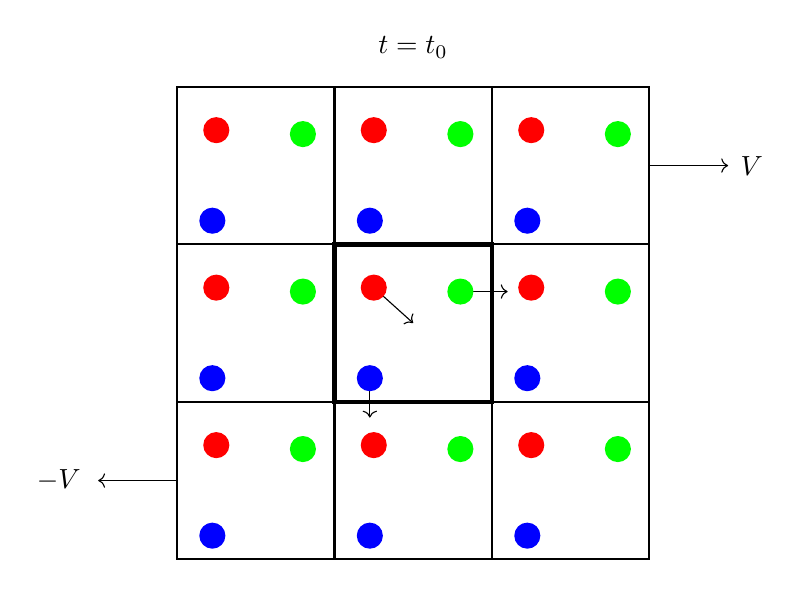
\begin{tikzpicture}

\draw[->](7.45,3.3)--(7.45,2.8);
 \draw[->](8.6,4.4)--(9.2,4.4);
  \draw[->](7.5,4.45)--(8,4);
    
\foreach \x in {5,7,9} {
    \foreach \y in {1,3,5} {
        \node[circle, fill=blue] at (\x+0.45,\y+0.3) {};
        \node[circle, fill=green] at (\x+1.6 ,\y+1.4) {};
        \node[circle, fill=red] at (\x+0.5 ,\y+1.45) {};
        
        % edge of each box
        \path[draw,thick] (\x,\y) rectangle (\x+2,\y+2);
    }
}


\path[draw,ultra thick] (7,3) rectangle (9,5);
 \draw[->](5,2)--(4,2);

  \draw(3.5,2)node{$-V$};
  
 \draw[->](11,6)--(12,6);
  \draw(12.3,6)node{$V$};
  
  \draw(8,7.5)node{$t=t_0$};
\end{tikzpicture}%
\end{document}